\documentclass{standalone}
\usepackage{tikz}
\usetikzlibrary{patterns, positioning}
\usepackage[sfdefault]{ClearSans} %% option 'sfdefault' activates Clear Sans as the default text font
\usepackage[T1]{fontenc}

\begin{document}
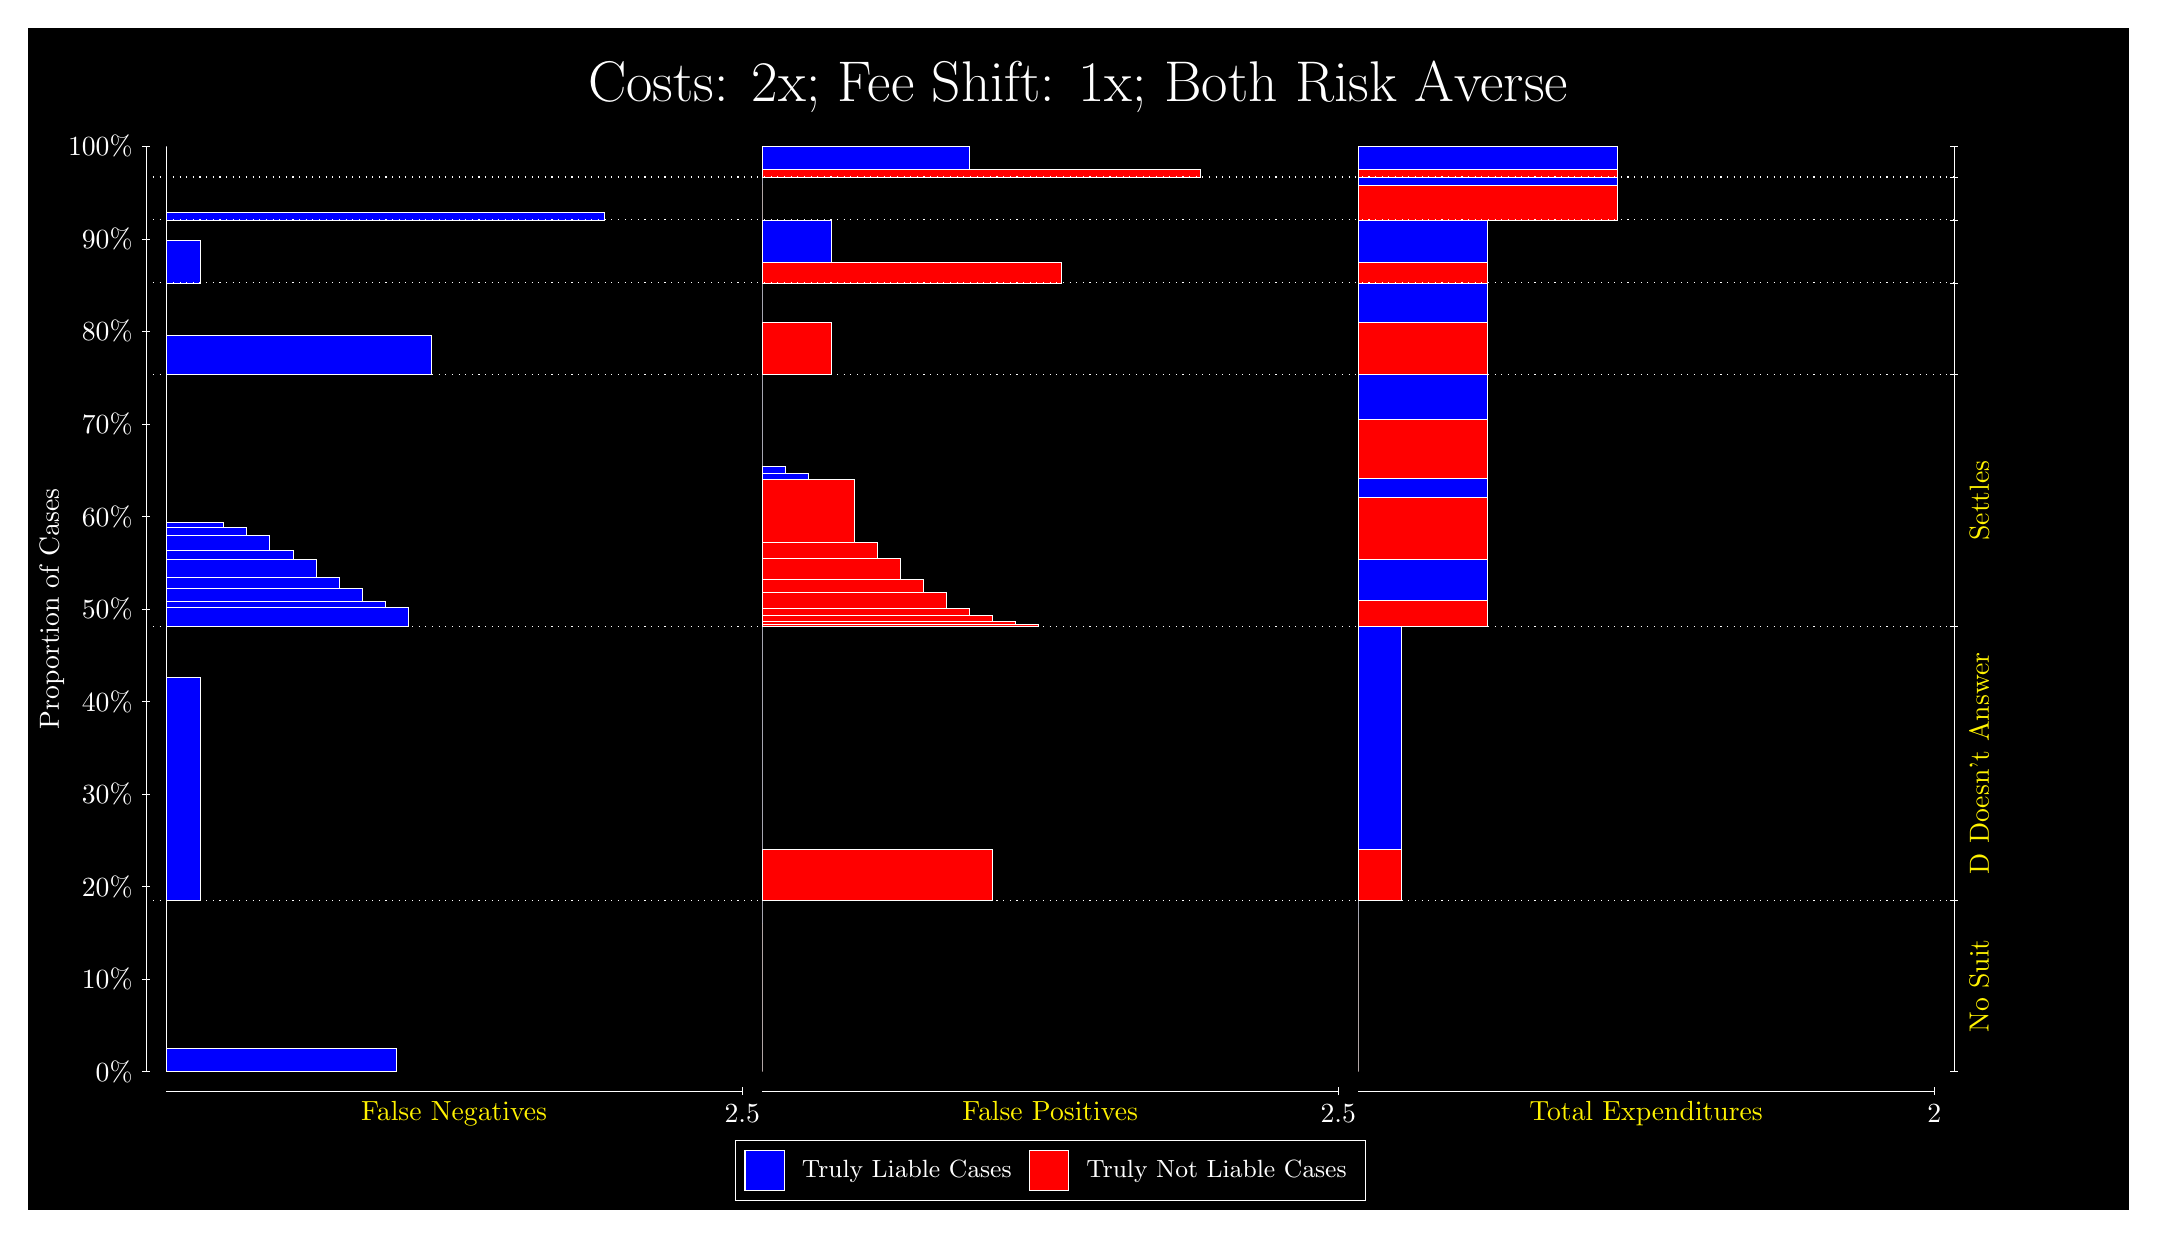
\begin{tikzpicture}
\draw[fill=black] (0,0) rectangle (26.667,15);
\draw[text=white] (0,13.5) rectangle (26.667,15) node[midway] {\huge Costs: 2x; Fee Shift: 1x; Both Risk Averse};
\draw[white, very thin] (1.5,1.75) -- (1.5,13.5);
\node[rotate=90, text=white, anchor=center] at (0.3, 7.625) {Proportion of Cases};
\draw[white, very thin] (1.45,1.75) -- (1.55,1.75);
\node[text=white, anchor=east] at (1.45, 1.75) {0\%};
\draw[white, very thin] (1.45,2.925) -- (1.55,2.925);
\node[text=white, anchor=east] at (1.45, 2.925) {10\%};
\draw[white, very thin] (1.45,4.1) -- (1.55,4.1);
\node[text=white, anchor=east] at (1.45, 4.1) {20\%};
\draw[white, very thin] (1.45,5.275) -- (1.55,5.275);
\node[text=white, anchor=east] at (1.45, 5.275) {30\%};
\draw[white, very thin] (1.45,6.45) -- (1.55,6.45);
\node[text=white, anchor=east] at (1.45, 6.45) {40\%};
\draw[white, very thin] (1.45,7.625) -- (1.55,7.625);
\node[text=white, anchor=east] at (1.45, 7.625) {50\%};
\draw[white, very thin] (1.45,8.8) -- (1.55,8.8);
\node[text=white, anchor=east] at (1.45, 8.8) {60\%};
\draw[white, very thin] (1.45,9.975) -- (1.55,9.975);
\node[text=white, anchor=east] at (1.45, 9.975) {70\%};
\draw[white, very thin] (1.45,11.15) -- (1.55,11.15);
\node[text=white, anchor=east] at (1.45, 11.15) {80\%};
\draw[white, very thin] (1.45,12.325) -- (1.55,12.325);
\node[text=white, anchor=east] at (1.45, 12.325) {90\%};
\draw[white, very thin] (1.45,13.5) -- (1.55,13.5);
\node[text=white, anchor=east] at (1.45, 13.5) {100\%};

\draw[white, very thin] (24.457,1.75) -- (24.457,13.5);
\draw[white, very thin] (24.407,1.75) -- (24.507,1.75);
\node[anchor=west] at (24.407, 1.75) {};
\draw[white, very thin] (24.407,3.9261) -- (24.507,3.9261);
\node[anchor=west] at (24.407, 3.9261) {};
\draw[white, very thin] (24.407,7.4013) -- (24.507,7.4013);
\node[anchor=west] at (24.407, 7.4013) {};
\draw[white, very thin] (24.407,10.6) -- (24.507,10.6);
\node[anchor=west] at (24.407, 10.6) {};
\draw[white, very thin] (24.407,11.767) -- (24.507,11.767);
\node[anchor=west] at (24.407, 11.767) {};
\draw[white, very thin] (24.407,12.567) -- (24.507,12.567);
\node[anchor=west] at (24.407, 12.567) {};
\draw[white, very thin] (24.407,13.111) -- (24.507,13.111);
\node[anchor=west] at (24.407, 13.111) {};
\draw[white, very thin] (24.407,13.5) -- (24.507,13.5);
\node[anchor=west] at (24.407, 13.5) {};

\draw[white, very thin, fill=blue] (1.75,1.75) rectangle (4.6775,2.0416);
\draw[white, very thin, fill=red] (1.75,2.0416) rectangle (1.75,3.9261);
\draw[white, very thin, fill=blue] (1.75,3.9261) rectangle (2.1891,6.7554);
\draw[white, very thin, fill=red] (1.75,6.7554) rectangle (1.75,7.4013);
\draw[white, very thin, fill=blue] (1.75,7.4013) rectangle (4.8239,7.641);
\draw[white, very thin, fill=blue] (1.75,7.641) rectangle (4.5312,7.7172);
\draw[white, very thin, fill=blue] (1.75,7.7172) rectangle (4.2384,7.8854);
\draw[white, very thin, fill=blue] (1.75,7.8854) rectangle (3.9457,8.023);
\draw[white, very thin, fill=blue] (1.75,8.023) rectangle (3.6529,8.2571);
\draw[white, very thin, fill=blue] (1.75,8.2571) rectangle (3.3602,8.3707);
\draw[white, very thin, fill=blue] (1.75,8.3707) rectangle (3.0674,8.5664);
\draw[white, very thin, fill=blue] (1.75,8.5664) rectangle (2.7746,8.6585);
\draw[white, very thin, fill=blue] (1.75,8.6585) rectangle (2.4819,8.7304);
\draw[white, very thin, fill=red] (1.75,8.7304) rectangle (1.75,10.6);
\draw[white, very thin, fill=blue] (1.75,10.6) rectangle (5.1167,11.098);
\draw[white, very thin, fill=red] (1.75,11.098) rectangle (1.75,11.767);
\draw[white, very thin, fill=blue] (1.75,11.767) rectangle (2.1891,12.305);
\draw[white, very thin, fill=red] (1.75,12.305) rectangle (1.75,12.567);
\draw[white, very thin, fill=blue] (1.75,12.567) rectangle (7.3123,12.667);
\draw[white, very thin, fill=red] (1.75,12.667) rectangle (1.75,13.111);
\draw[white, very thin, fill=red] (1.75,13.111) rectangle (1.75,13.211);
\draw[white, very thin, fill=blue] (1.75,13.211) rectangle (1.75,13.5);
\draw[white, very thin, fill=red] (9.3189,1.75) rectangle (9.3189,3.6345);
\draw[white, very thin, fill=blue] (9.3189,3.6345) rectangle (9.3189,3.9261);
\draw[white, very thin, fill=red] (9.3189,3.9261) rectangle (12.246,4.572);
\draw[white, very thin, fill=blue] (9.3189,4.572) rectangle (9.3189,7.4013);
\draw[white, very thin, fill=red] (9.3189,7.4013) rectangle (12.832,7.4245);
\draw[white, very thin, fill=red] (9.3189,7.4245) rectangle (12.539,7.4625);
\draw[white, very thin, fill=red] (9.3189,7.4625) rectangle (12.246,7.5447);
\draw[white, very thin, fill=red] (9.3189,7.5447) rectangle (11.954,7.6292);
\draw[white, very thin, fill=red] (9.3189,7.6292) rectangle (11.661,7.8381);
\draw[white, very thin, fill=red] (9.3189,7.8381) rectangle (11.368,8.0062);
\draw[white, very thin, fill=red] (9.3189,8.0062) rectangle (11.075,8.2714);
\draw[white, very thin, fill=red] (9.3189,8.2714) rectangle (10.783,8.4753);
\draw[white, very thin, fill=red] (9.3189,8.4753) rectangle (10.49,9.2711);
\draw[white, very thin, fill=blue] (9.3189,9.2711) rectangle (9.9044,9.3429);
\draw[white, very thin, fill=blue] (9.3189,9.3429) rectangle (9.6116,9.435);
\draw[white, very thin, fill=blue] (9.3189,9.435) rectangle (9.3189,10.6);
\draw[white, very thin, fill=red] (9.3189,10.6) rectangle (10.197,11.27);
\draw[white, very thin, fill=blue] (9.3189,11.27) rectangle (9.3189,11.767);
\draw[white, very thin, fill=red] (9.3189,11.767) rectangle (13.125,12.029);
\draw[white, very thin, fill=blue] (9.3189,12.029) rectangle (10.197,12.567);
\draw[white, very thin, fill=red] (9.3189,12.567) rectangle (9.3189,13.011);
\draw[white, very thin, fill=blue] (9.3189,13.011) rectangle (9.3189,13.111);
\draw[white, very thin, fill=red] (9.3189,13.111) rectangle (14.881,13.211);
\draw[white, very thin, fill=blue] (9.3189,13.211) rectangle (11.954,13.5);
\draw[white, very thin, fill=red] (16.888,1.75) rectangle (16.888,3.6345);
\draw[white, very thin, fill=blue] (16.888,3.6345) rectangle (16.888,3.9261);
\draw[white, very thin, fill=red] (16.888,3.9261) rectangle (17.437,4.572);
\draw[white, very thin, fill=blue] (16.888,4.572) rectangle (17.437,7.4013);
\draw[white, very thin, fill=red] (16.888,7.4013) rectangle (18.534,7.7304);
\draw[white, very thin, fill=blue] (16.888,7.7304) rectangle (18.534,8.2523);
\draw[white, very thin, fill=red] (16.888,8.2523) rectangle (18.534,9.0481);
\draw[white, very thin, fill=blue] (16.888,9.0481) rectangle (18.534,9.2877);
\draw[white, very thin, fill=red] (16.888,9.2877) rectangle (18.534,10.033);
\draw[white, very thin, fill=blue] (16.888,10.033) rectangle (18.534,10.6);
\draw[white, very thin, fill=red] (16.888,10.6) rectangle (18.534,11.27);
\draw[white, very thin, fill=blue] (16.888,11.27) rectangle (18.534,11.767);
\draw[white, very thin, fill=red] (16.888,11.767) rectangle (18.534,12.029);
\draw[white, very thin, fill=blue] (16.888,12.029) rectangle (18.534,12.567);
\draw[white, very thin, fill=red] (16.888,12.567) rectangle (20.181,13.011);
\draw[white, very thin, fill=blue] (16.888,13.011) rectangle (20.181,13.111);
\draw[white, very thin, fill=red] (16.888,13.111) rectangle (20.181,13.211);
\draw[white, very thin, fill=blue] (16.888,13.211) rectangle (20.181,13.5);
\draw[white, dotted] (1.5,3.9261) -- (24.457,3.9261);
\draw[white, dotted] (1.5,7.4013) -- (24.457,7.4013);
\draw[white, dotted] (1.5,10.6) -- (24.457,10.6);
\draw[white, dotted] (1.5,11.767) -- (24.457,11.767);
\draw[white, dotted] (1.5,12.567) -- (24.457,12.567);
\draw[white, dotted] (1.5,13.111) -- (24.457,13.111);
\draw[white, very thin] (1.75,1.5) -- (9.0689,1.5);
\node[text=yellow, anchor=north] at (5.4094, 1.5) {False Negatives};
\draw[white, very thin] (9.0689,1.45) -- (9.0689,1.55);
\node[text=white, anchor=north] at (9.0689, 1.45) {2.5};

\draw[white, very thin] (9.3189,1.5) -- (16.638,1.5);
\node[text=yellow, anchor=north] at (12.978, 1.5) {False Positives};
\draw[white, very thin] (16.638,1.45) -- (16.638,1.55);
\node[text=white, anchor=north] at (16.638, 1.45) {2.5};

\draw[white, very thin] (16.888,1.5) -- (24.207,1.5);
\node[text=yellow, anchor=north] at (20.547, 1.5) {Total Expenditures};
\draw[white, very thin] (24.207,1.45) -- (24.207,1.55);
\node[text=white, anchor=north] at (24.207, 1.45) {2};

\node[text=yellow, centered, rotate=90] at (24.777, 2.838) {No Suit};
\node[text=yellow, centered, rotate=90] at (24.777, 5.6637) {D Doesn't Answer};
\node[text=yellow, centered, rotate=90] at (24.777, 9.0007) {Settles};





\draw (12.978300999999998,1.5) node[draw=none] (baseCoordinate) {};
\begin{scope}[align=center]
        \matrix[scale=0.5, draw=white, below=0.5cm of baseCoordinate, nodes={draw}, column sep=0.1cm]{
            \node[rectangle, draw, minimum width=0.5cm, minimum height=0.5cm, fill=blue] {}; &
            \node[draw=none, font=\small, text=white] (B) {Truly Liable Cases}; &
            \node[rectangle, draw, minimum width=0.5cm, minimum height=0.5cm, fill=red] {}; &
            \node[draw=none, font=\small, text=white] (B) {Truly Not Liable Cases}; \\
            };
\end{scope}

\end{tikzpicture}
\end{document}